\begin{frame}{}
%{Kilonova afterglow for \GRB{} rebrightening$^{\text{\citep{Hajela:2021faz,Nedora:2021eoj}}}$} %% ---------- title 
\begin{tikzpicture}[overlay,remember picture]

\uncover<1->{ % <-> |
    \node (img1) [anchor=center,scale=1,opacity=1] at ([shift={(-3.5cm,3.1cm)}]current page.center){
        \parbox{0.6\textwidth}{
            \small{\textbf{Changing afterglow of \GW{}}} \\
            \tiny{ Hajela...VN+21 \textcolor{gray}{arXiv:2104.02070} }
    }};
}

\uncover<1->{ % <-> |
    \node (img1) [anchor=center,scale=1,opacity=1] at ([shift={(-4.0cm,1.0cm)}]current page.center){
        \parbox{0.5\textwidth}{
            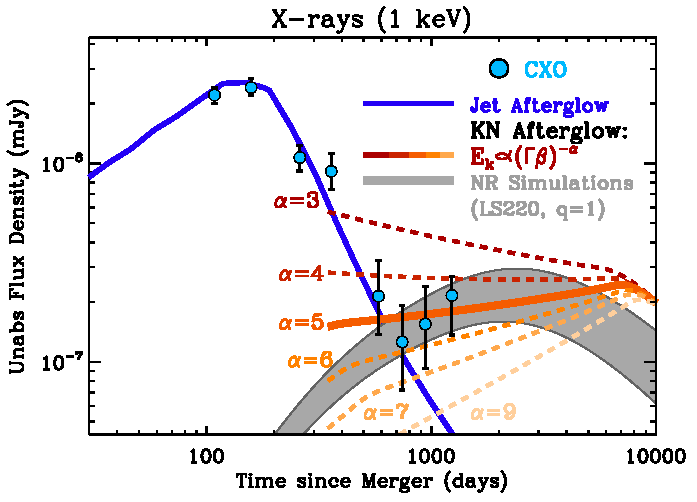
\includegraphics[height=3.7cm]{Hajela_VN_21_kn_afterglow2.pdf}
    }};
}





\uncover<1->{ % <-> |
    \node (t1) [anchor=center,scale=1,opacity=1] at ([shift={(-2.8cm,-2.5cm)}]current page.center){
        \parbox{0.7\textwidth}{
            Possible explanations:
            \begin{itemize}
            \item Change in ISM
            \item Evolution of the shock microphayics parameters
            \item New emission component (fall-back accretion, kilonova afterglow)
            \end{itemize}
    }};
}

%\uncover<1->{ % <-> |
%    \node (img1) [anchor=center,scale=1,opacity=1] at ([shift={(-4.0cm,-1.5cm)}]current page.center){
%        \parbox{0.5\textwidth}{
%            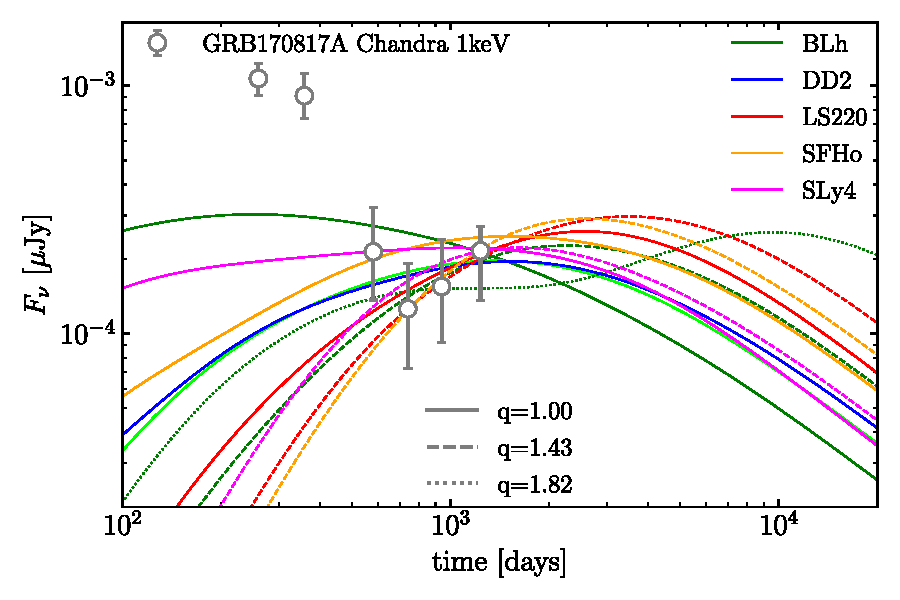
\includegraphics[height=5cm]{kn_afterglow/best_xray_obs_representative_all_eos.pdf}
%    }};
%}

%\uncover<1->{ % <-> |
%    \node (img1) [anchor=center,scale=1,opacity=1] at ([shift={(4.0cm,2.1cm)}]current page.center){
%        \parbox{0.5\textwidth}{
%            \includegraphics[height=3.5cm]{Hajela_VN_21_kn_afterglow.pdf}
%    }};
%}
\uncover<1->{ % <-> |
    \node (img1) [anchor=center,scale=1,opacity=1] at ([shift={(4.0cm,2.6cm)}]current page.center){
        \parbox{0.7\textwidth}{
            Considering KN afterglow (\texttt{PyBlastAfterglow}):
            \begin{itemize}
                \item NR-informed kN afterglow consisent with observations 
                \item New propspect to constrain BNS parameters
            \end{itemize}
    }};
}
\uncover<1->{ % <-> |
    \node (img1) [anchor=center,scale=1,opacity=1] at ([shift={(4.8cm,1.0cm)}]current page.center){
        \parbox{0.5\textwidth}{
            \small{\textbf{NR-informed LCs from Dyn.Ej}} \\
            \tiny{ VN+21 \textcolor{gray}{arXiv:2104.04537} }
    }};
}
\uncover<1->{ % <-> |
    \node (img1) [anchor=center,scale=1,opacity=1] at ([shift={(4.8cm,-1.8cm)}]current page.center){
        \parbox{0.5\textwidth}{
            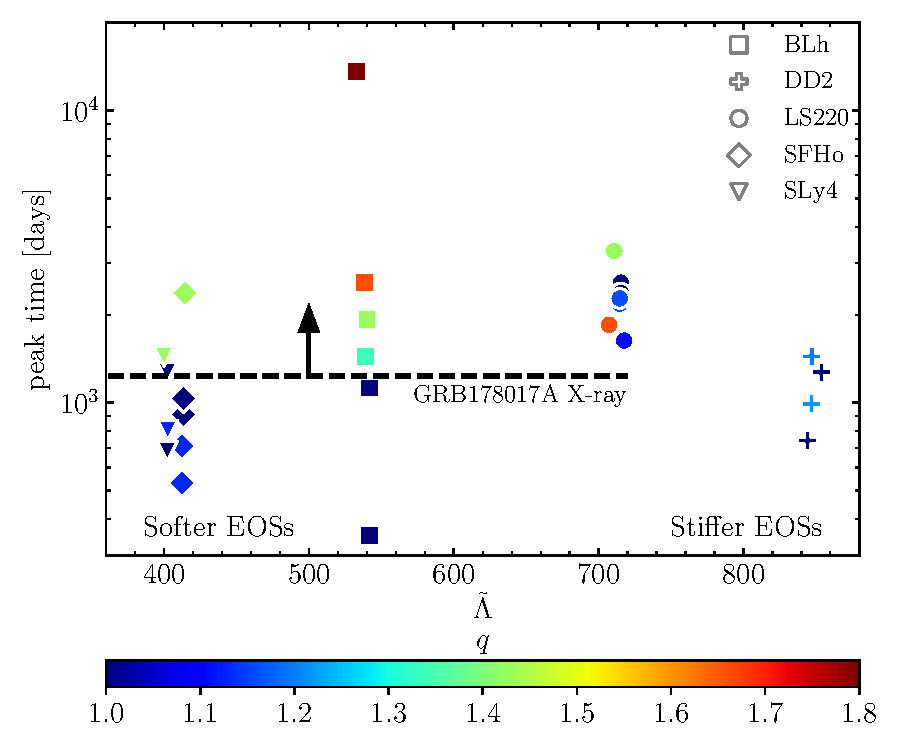
\includegraphics[height=4.8cm]{kn_afterglow/scatter_lightcurve_tpeak_vs_lambda.pdf}
    }};
}

\end{tikzpicture}

\end{frame}